%% 和文論文用のテンプレート
%%%%%%%%%%%%%%%%%%%%%%%%%%%%%%%%%%%%%%%%%%%%%%%%%%%%%%%%%%%%%%%%%%%%%%%%%%%%
%% 1. 和文原稿
\documentclass[originalpaper,dvipdfmx]{jsaiart}     % 原著論文 Original Paper
% \documentclass[shortpaper]{jsaiart}       % 速報論文 Short Paper
% \documentclass[exploratorypaper]{jsaiart} % 萌芽論文 Exploratory Research Paper
% \documentclass[Specialissue]{jsaiart}     % 特集 Special Issue
% \documentclass[specialissue]{jsaiart}     % 小特集 Special Issue
% \documentclass[interimreport]{jsaiart}    % 報告 An Interim Report
% \documentclass[surveypaper]{jsaiart}      % 解説 Survey Paper
% \documentclass[aimap]{jsaiart}            % AIマップ AI map
% \documentclass[specialpaper]{jsaiart}     % 特集論文 Special Paper
% \documentclass[invitedpaper]{jsaiart}     % 招待論文 Invited Paper
%
% %% 2023年 single-blind 化により [blind] オプションは無効化しました
%

%% ページ番号の指定，掲載時に学会の方で決定します．
% \setcounter{page}{1}
% \setcounter{volpage}{1}


%%% amsmathパッケージの注意点 %%%%%%%%%%%%%%%%%%%%%%%%%%%%%%%%%%%%%%%
% \usepackpage{amsmath}
% 数式番号の参照は \ref ではなく，\eqref を用いること
% documentclass のオプションに fleqnを指定すること
% 例: \documentclass[technicalpaper,fleqn]{jsaiart}

\usepackage[dvipdfmx]{graphicx}
% \usepackage[dvips]{graphicx}
\usepackage{pifont}
\usepackage{profile-2e}
\usepackage{amsmath}
\usepackage{amssymb}
\usepackage{array} 
\usepackage{bm}
\usepackage{xcolor}
\usepackage{subfig}
\usepackage{colortbl}
\usepackage[utf8]{inputenc}
\usepackage{url}
\usepackage[dvipdfmx,hidelinks]{hyperref}
\usepackage{pxjahyper}
\usepackage{otf}
\usepackage{remreset}
\usepackage {booktabs}
\usepackage {diagbox}
\newcolumntype{P}[1]{>{\centering\arraybackslash}m{#1}}
\usepackage{doi}
\usepackage{caption}
\captionsetup{compatibility=false} 
\usepackage{multirow}
\usepackage{siunitx}
\usepackage{pdfpages}
\usepackage{threeparttable}
\usepackage{arydshln}
\usepackage{xurl}
\Vol{1}
\No{2}
\jtitle{コストと精度を考慮した質問と文書の特徴に基づく適応的なRAG構成選択}
% コストと精度を考慮した質問と文書の特徴に基づく適応的なRAG選択
% \jtitle[柱用和文タイトル]{和文タイトル}
% \jsubtitle{和文サブタイトル}
\etitle{Adaptive RAG Configuration Selection Based on Question and Document Features Considering Cost and Accuracy}
% Adaptive RAG Configuration Selection Based on Question and Document Features Considering Cost and Accuracy
% \esubtitle{英文サブタイトル}

\manyauthor % 著者が3名以下の場合はこの行を消すこと

%%% 著者名の注意点 %%%%%%%%%%%%%%%%%%%%%%%%%%%%%%%%%%%%%%%%%%%%%%%%%%%
% 所属先が同じ著者が連続する場合，その中の先頭の著者のみ \affiliation
% を用い，残りの所属先には \sameaffiliation を使う
% ただし，所属先が同じでも連続していない場合は \affliation を使う
% 名前が長い場合は \name の代りに \longname を使う

\author{%
 \name{穴口}{史将}{Fumikatsu Anaguchi}
 \affiliation{青山学院大学，産業技術総合研究所}%
     {Aoyama Gakuin University, National Institute of Advanced Industrial Science and Technology}%
     {}
\and
 \longname{チャクラボルティ}{シュデシナ}{Sudesna Chakraborty}
 \affiliation{青山学院大学}%
     {Aoyama Gakuin University}%
     {}
\and
 \name{森田}{武史}{Takeshi Morita}
 \affiliation{青山学院大学，産業技術総合研究所}%
     {Aoyama Gakuin University, National Institute of Advanced Industrial Science and Technology}%
     {morita@it.aoyama.ac.jp}
\and
\name{太田}{葵}{Aoi Ohta}
 \affiliation{産業技術総合研究所}%
     {National Institute of Advanced Industrial Science and Technology}%
     {}
     \and
\name{浅田}{真生}{Masaki Asada}
 \sameaffiliation{}
\and
 \name{江上}{周作}{Shusaku Egami}
 \sameaffiliation{}
\and
 \name{鵜飼}{孝典}{Takanori Ugai}
 \affiliation{富士通株式会社，産業技術総合研究所}%
     {Fujitsu Limited, National Institute of Advanced Industrial Science and Technology}%
     {}
     \and
\name{濱崎}{雅弘}{Masahiro Hamasaki}
 \affiliation{産業技術総合研究所}%
     {National Institute of Advanced Industrial Science and Technology}%
     {}
}
% masahiro.hamasaki@aist.go.jp

\begin{keyword}
% キーワードとして，小文字（固有名詞や略語を除く）の英単語を2〜5個指定
retrieval-augmented generation， graph-based RAG， adaptive RAG， learning to rank， large language model
\end{keyword}

\begin{summary}
% 「ショートノート」は 200 ワード，それ以外は200〜500 ワード
% 以内の英文でsummaryを記す
Large Language Models (LLMs) face the challenge of generating misinformation or hallucinating about facts absent from their training data. Retrieval-Augmented Generation (RAG) addresses this by incorporating external knowledge sources. However, different queries require different RAG configurations; while complex queries benefit from high-cost strategies (e.g., GraphRAG), simple queries can be resolved using fast, low-cost configurations (e.g., NaiveRAG). Consequently, adaptive RAG systems are essential for balancing quality and computational cost. Existing adaptive RAG approaches often rely on LLMs to route queries, introducing significant runtime overhead, or use online reinforcement learning, which incurs ongoing operational costs. Moreover, unified frameworks optimizing multi-objective trade-offs (e.g., accuracy and latency) across heterogeneous configurations (e.g., chunk size, embedders, generators) are lacking. This study proposes an offline, learning-to-rank approach for adaptive RAG configuration selection. We train a ranking model using multi-faceted query and document features to rank 96 candidate RAG configurations. During inference, candidate configurations are ranked without LLM-overhead, and the optimal configuration is selected based on user-defined priority weights for precision, recall, F1-score, and execution time. Evaluation results show that our method outperforms standard baselines, achieving significant Pareto improvements. Specifically, our balanced configuration achieves a 14.15% point improvement in BERTScore F1-score and an 86.2% reduction in execution time compared to the state-of-the-art Adaptive-RAG baseline. Furthermore, Wilcoxon signed-rank tests confirm the statistical significance of our approach.
\end{summary}


\begin{document}
\maketitle

\section{はじめに} \label{sec1}
% Llama3.1~\cite{Meta24}やQwen3~\cite{qwen25}のような大規模言語モデル（Large Language Model, LLM）は，多様なタスクで高い性能を発揮している~\cite{zhao25}．
% Llama3.1~\cite{Meta24}やQwen3~\cite{qwen25}のような
Large Language Model（LLM）は多様なタスクで高い性能を発揮している~\cite{Zhao25}が，LLMの出力は学習データ内の知識に依存するため，未学習の知識に対して誤情報を生成する可能性がある~\cite{Ji23}．
また，日々更新される情報のすべてを網羅して学習することは困難である~\cite{Wang25}．
これらの課題に対する手法として，外部知識を検索し，その結果をLLMのコンテキストとして提示するRetrieval-Augmented Generation（RAG）~\cite{Lewis20}が提案されている．
RAGにより，LLMは最新かつ正確な知識を反映した応答が可能となる．

RAGの活用例の一つに，質問応答（Question Answering, QA）タスクがある．
RAGを用いたQAに関する初期の研究では，単一文書内に解答が存在するシングルホップ型のQAタスク~\cite{rajpurkar16}に焦点が当てられてきた~\cite{Shi24}．
しかし，複数文書間の関連付けや段階的推論を要する，マルチホップ型のQAタスクも多数存在する~\cite{yang18,ho20,trivedi22}．
例えば，「アインシュタインが相対性理論を発表したときのアメリカ大統領は誰ですか？」という質問は，発表時期と在任大統領を照合する二段階推論を必要とする．
このような複雑な質問に対応するため，LightRAG~\cite{Guo25}やGraphRAG~\cite{edge25}のようなマルチホップ型のQAタスクに焦点が当てられたRAGが提案されている．

一方で，これらの手法には，複数回の検索や段階的推論を必要とするため，推論時間が増大するという課題がある．
実運用において，入力される質問の全てが複雑であるとは限らない．
頻出する質問の中には単純かつ直接的なものも多く，例えば「アインシュタインの誕生日はいつですか？」のような質問は，外部検索を用いずともLLMの内部知識のみで回答できる場合がある~\cite{Mallen23}．
このような単純な質問に対しては，不要な検索や推論はコストを増大させるだけである．
%すなわち，複雑な質問には高精度なRAGが有効である一方，単純な質問に対しては不要な検索や推論がコストを増大させる．
しかし，複雑な質問を単純なRAG構成で処理した場合，回答精度が低下する可能性がある~\cite{LingjiaoChen24}．

% 研究課題
以上の背景から，質問の特徴に応じてRAGを動的に調整する「適応的なRAG」に関する研究が進展している~\cite{Asai23,fu24,Tang25,Rishi25,zhang2025adagcrag}．
% 具体的には，RAGのプロセス途中に検索の有無や関連文書の選択をLLMが調整する手法 ~\cite{Asai23}，オンライン強化学習によりハイパーパラメータや検索方法を最適化する手法~\cite{fu24,Tang25} ，質問に応じてファインチューニング済みモデルが検索方法を調整する手法~\cite{Rishi25}やハイパーパラメータを調整する手法~\cite{zhang2025adagcrag}も提案されている．
しかし，既存の適応的なRAGには，主に三つの課題がある．
    第一に，LLMの自己判定やプランニングを利用するエージェント指向の調整手法（Agentic RAG等）~\cite{Asai23}は，RAG構成の
決定にLLM自身の多段推論やオンライン探索を必要とする．そのため，回答精度が高まりやすい一方で，判断ごとに大きなLLM推論オー
バーヘッド（実行遅延やAPIコスト）が発生し，かつチャンクサイズや重複度といった複数のミクロなハイパーパラメータを総合的か
つ低コストに調整することが困難である．
    第二に，オンライン強化学習を用いた手法~\cite{fu24,Tang25}は，稼働中の環境での継続的な試行錯誤と学習を伴うため，実運用時のインフラコストや学習の不確実性が高まりやすい．
    第三に，質問や文書の特徴に基づく適応的アプローチ~\cite{Rishi25,zhang2025adagcrag}は存在するが，それらの多くはマクロな処理パラダイムの切り替え（例: 検索有無やモデルの動的ルーティング）や特定のグラフベースRAGパラメータの制御に特化しており，多様なRAG方式（Graph / Non-Graph）を横断し，かつチャンクサイズや重複度といったミクロなハイパーパラメータまでを含めた大規模な離散構成空間（全96通り）を一括して順位付けするアプローチは十分に議論されていない．また，対立する多目的指標（適合率，再現率，F1値，実行時間）を実行時にユーザ定義の優先度（重み $W$）に応じて動的に制御できる統合的なフレームワークも限られている．

% 研究目的
これらの課題に対し，本研究はLLMやオンラインでの継続的な学習・探索に依存せず，事前に収集した実測データから多様なRAG構成を学習するオフライン学習を採用する．
推論時に追加のLLM推論を必要とする調整ではなく，あらかじめ定義したRAG構成空間の候補に対して，精度指標とコスト指標それぞれのランキングを学習し，推論時は学習済みランキングモデル（Ranking Model, RM）の推論と任意の重みでRAG構成を選択する．
これにより，オンライン探索を伴うエージェント指向の調整手法と比較して，推論コストと応答遅延（ミリ秒オーダーの決定）を大幅に抑えつつ，複数のRAGとハイパーパラメータを含む広い構成空間を一括して扱うことを目指す．
また，オンライン学習を前提としないため，第二の課題である運用時の継続的な学習コストも回避する．
さらに，質問側の特徴に加えて文書側の表層的特徴および意味的特徴を用い，精度指標とコスト指標を統合した多目的な観点から学習することで，第三の課題に対応する．

% 手法概説
本手法では，まず質問と文書から統計量に基づく表層的特徴および埋め込み表現に基づく意味的特徴を抽出する．
学習時には，多様な RAG 構成に対する実測性能を教師データとしてRMを学習する．
% 実測性能（適合率，再現率，$F_1$ 値，時間）
推論時には，このRMが各質問に対して候補構成を順位付けし，上位の構成を選択することで，低コストや高精度のRAG構成を選択する．
さらに，精度重視，バランス重視，コスト重視といった要求に応じて重み付けを切り替え，複数のランキング結果を使い分けることで，ユーザの多様な要求に対応する．

% 実験概説
評価実験では，QAタスクを対象として，RMの性能と，本手法により選択されたRAG構成を用いた最終的な応答を評価する．
%実験の結果，ランキングモデルはランダムと比較して高い精度で順位を予測できており，特に時間の予測において優れた性能を示した．
%また，本手法によって択されたRAG構成は，質問に対して同一の RAG 構成を適用した場合と比較して， $F_1$値 を改善しつつ時間を短縮した．
%加えて，精度とコストのトレードオフを運用方針に応じて調整できることを確認した．
%さらに，ユーザ選択を含む適応的なRAG構成選択を用いた実験では，本手法の実用性が示され，特に時間重視の設定ではオラクルと同等の性能に到達した．

本研究の貢献は以下の通りである．
\begin{itemize}
\item RAG構成情報（生成モデルや検索方式等）が順位付けの基盤となる一方，質問・文書の表層的および意味的特徴量を包括的に統合することで，構成単独（NDCG@1=66.84\%）を上回る最高精度（NDCG@1=68.52\%，Hit@5=65.00\%）のランキングが可能となることを実験的に明らかにした．
\item 精度（適合率，再現率，$F_1$値）とコスト（実行時間）を統合的に扱う多目的ランキング手法を導入し，ユーザの優先順位や入力状況に応じたRAG構成の適応的な自動選択を実現した．
\end{itemize}

% \item 質問および文書の表層的特徴と意味的特徴を統合したRAG構成選択用の特徴量を設計し，それらを考慮したランキングモデルを構築した．
% \item 精度（適合率，再現率，$F_1$値）とコスト（時間）を統合的に評価する多目的ランキング手法を導入し，ユーザの要求に応じて適応的なRAG構成を選択する手法を提案した．
本論文の構成は次の通りである．
第~\ref{sec2}では本研究の関連研究を概説し，第~\ref{sec3}では提案手法について詳述する.
第~\ref{sec4}では評価実験の方法について述べ，第~\ref{sec5}では評価実験結果および考察を述べる．
最後に，第~\ref{sec6}では本研究の結論と今後の課題を提示する．

なお，本論文は，穴口らの研究成果~\cite{anaguchi26}に対し，以下の具体的な追加・拡張を行ったものである．
第一に，近接研究（CARROT，uRAG，RAGRouter，AdaGCRAG）との関係性を整理し，手法のポジショニングを明確化した．
第二に，既存の代表的な適応的RAGベースライン手法であるAdaptive-RAGを評価フレームワークに組み込み，精度とコストのParetoフロンティアの観点から性能評価を行った．
第三に，自動評価指標（BERTScore）に加えて，標準的QA評価指標であるExact Match (EM)およびToken-level $F_1$値を用いて提案手法を多角的に再評価した．
第四に，提案手法とベースライン間の差について，Wilcoxon符号付き順位検定による有意差検定を行い，回答精度の統計的優位性を立証した．
最後に，上位K件提示モデルにおける構成順次試行コストを「累積実行時間」として計上し，より実用的なコスト効率性を実証した．
\section{関連研究} \label{sec2}
% \subsection{Retrieval-Augmented Generation (RAG)} \label{sec2.1}
% \subsection{適応的なRAG} \label{sec2.2}
質問の特徴に適応して検索方法やハイパーパラメータを選択する，適応的なRAGに関する研究が進展している~\cite{Asai23,fu24,Tang25,Rishi25,Zhang25}．
一般に，複雑な質問にはグラフベースRAG等の高精度な手法が有効である一方，単純な質問に複雑な処理を適用すると，不要な検索や計算によりコストが増大する．
一方，複雑な質問をNaiveRAGのような単純な手法や非検索で処理した場合には，応答品質が低下する~\cite{Jeong24}． 
適応的なRAGは，質問の複雑さに応じて検索方法やハイパーパラメータを選択し，応答品質の向上を目指す．

既存研究の多くは，LLMによる自己判定やオンライン強化学習に基づいている．
Self-RAG~\cite{Asai23}は，RAGの検索方法をLLMが自己評価しながら生成する手法である．
AutoRAG-HP~\cite{fu24}は，RAGの性能の要因となる複数のハイパーパラメータをオンライン強化学習で最適化する手法である．
Tangら~\cite{Tang25}は，グラフベースRAGにおいて，質問の特性に応じて最適な検索手法を自動的に選択する手法を提案した．
また，HyPA-RAG~\cite{Rishi25}は，質問の特性に応じて複数のハイパーパラメータを動的に最適化する手法である．
AdaGCRAG~\cite{Zhang25}は，小規模言語モデル環境においても高い性能と効率性を両立させる手法である．
これらの適応的なRAGは，検索方法の判断やバンディットによるオンライン最適化といった多様なアプローチにより実現されている．

これに対し，本研究では，質問と文書の多面的な特徴量および過去の評価結果に基づき，候補となるRAG構成をRMにより直接順位付けする．
これにより，精度とコストのトレードオフを同時に考慮したRAG構成の自動選択を実現する．

\section{提案手法} \label{sec3}
\begin{figure}[tb]
\centerline{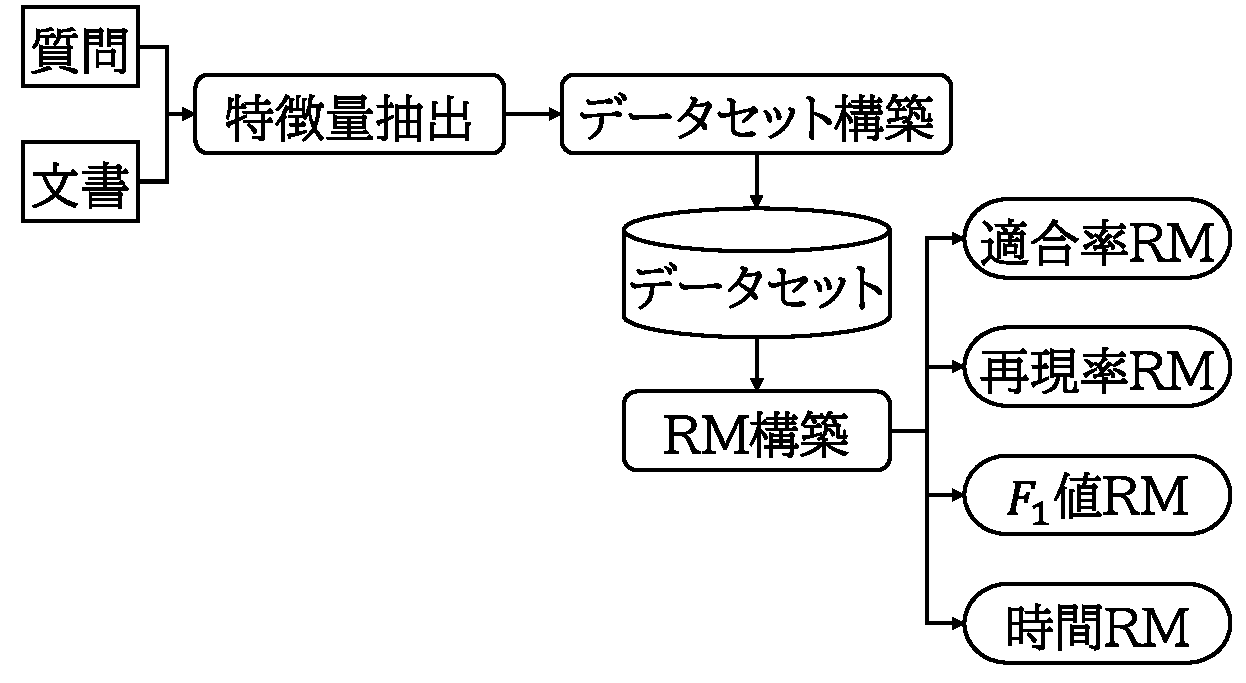
\includegraphics[width=\linewidth]{figures/method_construction_diagram.pdf}}
\caption{提案手法におけるランキングモデルの学習手順}
\label{construction}
\end{figure}

\begin{figure}[tb]
\centerline{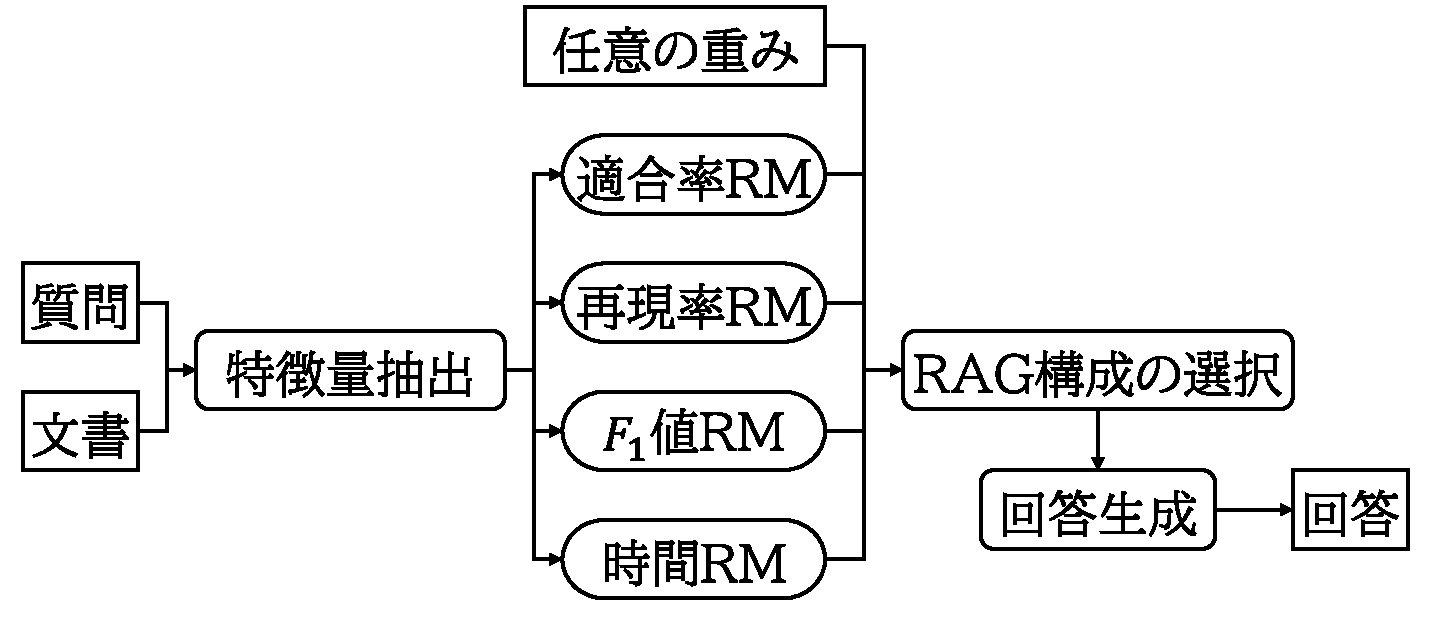
\includegraphics[width=\linewidth]{figures/method_reasoning_diagram.pdf}}
\caption{提案手法におけるランキングモデルの推論手順}
\label{reasoning}
\end{figure}

本研究では，質問と文書の特徴に応じてRAG構成を適応的に選択し，精度（適合率・再現率・$F_1$値）とコスト（実行時間）のトレードオフを調整する手法を提案する．
\ref{construction}および~\ref{reasoning}に，提案手法におけるRMの学習と推論の手順を示す．
%提案手法は，ランキングモデルの学習とランキングモデルによる推論により構成される．
% \ref{construction}および~\ref{reasoning}における適合率RM，再現率RM，$F_1$値RM，時間RMは，それぞれ適合率，再現率，$F_1$値，時間のRMを表す．
適合率RM，再現率RM，$F_1$値RM，時間RMは，質問と文書の特徴量とRAG構成を説明変数として用いる．
これらは，各RAG構成における適合率，再現率，$F_1$値，および実行時間の順位をそれぞれ予測するモデルである．
本章では，提案手法におけるRMの学習および推論の構成要素について述べる．

\subsection{特徴量抽出} \label{sec3.1}
本節では，質問および文書から表層的特徴量と意味的特徴量を抽出する方法を説明する． 
あらかじめ質問に関連する文書を一つ以上用意した上で，本処理はRMの学習と推論の双方で実行する． 
これらの特徴量は，質問の複雑さと意図，および質問と文書の関連性を捉えるために用いる． 
特徴量は，表層的特徴量4種類と意味的特徴量3種類の計7種類を選定した．
この選定は，事前に様々な特徴量の組み合わせを試し，RMの性能が最も向上する組を特定するというヒューリスティックな手法に基づいている．
なお，性能評価の詳細については，第~\ref{sec5.5}のアブレーション分析にて述べる．
% 特徴量は，ヒューリスティックな手法により，表層的特徴量4種類と意味的特徴量3種類の計7種類を選定した． 

\subsubsection{表層的特徴量の抽出}
表層的特徴量は，質問に関するトークン数，依存構造木の深さ，質問タイプ，および文書に関するトークン数の4種類である． 
質問のトークン数は，質問の表層的な長さを表すだけでなく，複数の条件，制約，あるいは修飾句を含む可能性を反映する指標である．
一般に，質問が長いほど，回答に必要な根拠が単一文書に収まらず，複数文書の統合を要する場合が増加する．

質問の依存構造木の深さは，トークン同士の係り受け関係を有向木として表現し，ルートトークンから深さ優先探索をした際の到達可能なパス長である．
木構造が深いほど修飾の入れ子や長距離依存が多く，文の解釈に必要な統合を要する場合が増加する．
RAG の構成選択の観点では，構文が複雑な質問ほど複数文書に跨る情報の統合を必要とする．

質問タイプは，期待される出力に基づき，真偽判定（Yes/No），本文抽出（事実情報の特定），選択（提示候補からの選定），文章生成（自由記述による説明）の4種類に分類する．
判定には，質問文の小文字化により得られた先頭語および特定語に基づくルールベースを採用する．
先頭語がis，can，mustといった助動詞やbe動詞である場合は，事象の成立可否を問う性質を持つため「真偽判定」に分類する．
一方，先頭語がwhat，who，whereといった疑問詞は，具体的な情報の特定を促すため「本文抽出」に分類する．
質問文に特定語（or）を含む場合は，選択を促す「選択」に分類する．
これら全条件に該当しない質問は，要約や理由説明の記述が求められるとみなし，「文章生成」に分類する．
% まず，真偽判定を促す語群（is, are, can, could, will, would, has, have, had, shall, should, may, might, must），選択を促す語（or），本文抽出を促す語群（what, who, when, where, which）のいずれに該当するかに基づいて，真偽判定，選択，本文抽出のいずれかに分類する．
% その他を説明生成や要約といった自由度の高い出力が求められるとみなし，文章生成に分類する．

文書に関するトークン数は，含まれる情報量の多さを示すと同時に，冗長性やノイズ量の増加を示唆する．
特に文書が長い場合，適切なチャンク分割の調整や検索後の統合手法の選択が性能およびコストに影響するため，本特徴量は構成選択に有用である．

\subsubsection{意味的特徴量の抽出}
意味的特徴量は，質問と文書の各埋め込み間のコサイン類似度，質問と文書から抽出したキーワードとの類似度，および質問と文書の双方から抽出した固有表現のコサイン類似度の3種類である．
質問と文書の各埋め込み間のコサイン類似度は，大域的な意味の一致度を測る指標であり，類似度が高い場合単一文書が回答根拠になり得る可能性が高く，比較的単純なRAG構成でも回答可能であると判断できる．

質問と文書から抽出したキーワードとの類似度は，質問と文書から抽出した語句を連結した文字列との類似度である．
文書は冗長な周辺情報を含みやすく，長文では質問に関連する箇所が埋もれる場合がある．
キーワードを用いることで要点レベルの整合性を判断する．
% そこで，文書からキーワードを抽出し，質問文との意味的近接性を測ることで要点レベルの整合性を評価する．

質問と文書の双方から抽出した固有表現のコサイン類似度は，質問および文書から抽出された固有表現の文字列を比較するものである．
固有表現は人物，組織，地名，作品名などの参照対象を表し，質問応答の品質を左右する要因となる．

以上の三つのコサイン類似度は，全文レベル，要点レベル，エンティティレベルという異なる観点から，質問と文書の関連性を補完的に捉えるものである．

\subsection{データセット構築} \label{sec3.2}
本節ではRMの学習，検証および評価に用いるデータセットの構築について述べる．
広範な構成空間から精度とコストの分布を系統的に取得し，RMが構成選択の規則性を学習する．
各質問に対して想定される全てのRAG構成を適用し，高精度な構成や低コストな構成を相対比較可能な順位ラベルを付与する．

RAG構成は，\ref{hyperparameters_in_RAG} に示す6項目の組み合わせからなる96通りに設定する．
RAGはNaiveRAG~\cite{Lewis20}，LightRAG~\cite{Guo25}，およびGraphRAG~\cite{edge25}を用いる． 
検索設定（Retrieval Setting, RS）は，NaiveRAGではStuffまたはMap Reduceとし，LightRAGおよびGraphRAGではローカル検索（Local）またはグローバル検索（Global）とする． 
チャンク設定は，NaiveRAGではチャンクサイズ（Chunk Size, CS）を250または500，チャンクオーバーラップ（Chunk Overlap, CO）を50または100とする． 
LightRAGおよびGraphRAGでは，CSを500または1000，COを100または250とする．
生成モデル（Generative Model, GM）には，Llama3.1:8b~\cite{Meta24}とQwen3:14b~\cite{qwen25} を用い，埋め込みモデル（Embedding Model, EM）にはnomic-embed-text~\cite{nussbaum25}とmxbai-embed-large~\footnote{\url{https://www.mixedbread.com/blog/} \url{mxbai-embed-large-v1/}}を用いる．
これにより多様な構成を網羅し，RM学習に必要な性能差を確保する．

なお，本研究では3種類のRAGを横断して比較可能な学習データを構築するため，構成の種類を可能な限り統一した．
% ただし，各RAGの構成は必ずしも同一ではない．
そのため，検索設定だけでなく，検索情報の統合方針（Chain Type）も広義の「検索設定」として扱う．
NaiveRAGにおけるChain Typeを，LightRAGおよびGraphRAGにおける検索設定と見なす．
本論文では，これらを統一して「検索設定」と記述する．

次に，各試行の結果として，質問 ID，RAG 構成，適合率，再現率，$F_1$値，実行時間を記録し，RMの特徴量と結合してデータセットを作成する．
具体的には，質問と文書を各 RAG 構成に入力し，得られた生成回答と正解を比較して BERTScore~\cite{zhang20}に基づく適合率・再現率・$F_1$ 値を算出する．
同時に，コストの指標として各試行の実行時間を計測する．
BERTScore は語彙の完全一致に依存せず，文脈埋め込みに基づいてトークン間の意味的対応を定量化できる．
そのため，表現の揺れを含む生成回答の評価に適している．
適合率，再現率，$F_1$値，実行時間には，相対的な順位を付与する．

% \begin{table*}[tb]
%     \centering
%     \small
%     % \footnotesize
%     \caption{RAG構成}
%     \label{hyperparameters_in_RAG}
% %    \resizebox{\columnwidth}{!}{
%     \begin{tabular}{cccccc}
%         \hline
%         \multirow{2}{*}{RAG} & \multirow{2}{*}{検索設定}
%         & \multicolumn{2}{c}{チャンク} & \multicolumn{2}{c}{モデル} \\
%         && サイズ & OL & 生成 & 埋め込み \\
%         \hline
%         \multirow{2}{*}{NaiveRAG} 
%         & Stuff & 250 & 50 & llama3.1:8b & nomic-embed-text \\
%         & MR & 500 & 100 & qwen3:14b & mxbai-embed-large \\
%         \hline
%         \multirow{2}{*}{LightRAG} 
%         & Local & 500 & 100 & llama3.1:8b & nomic-embed-text \\
%         & Global & 1000 & 250 & qwen3:14b & mxbai-embed-large \\
%         \hline
%         \multirow{2}{*}{GraphRAG} 
%         & Local & 500 & 100 & llama3.1:8b & nomic-embed-text \\
%         & Global & 1000 & 250 & qwen3:14b & mxbai-embed-large \\
%         \hline
%     \end{tabular}
% %    }
% \end{table*}

\begin{table}[tb]
    \centering
    \small
    % \footnotesize
    \caption{RAG構成（全96通りの組み合わせ）}
    \label{hyperparameters_in_RAG}
    \begin{tabular}{lll}
        \hline
        構成 & 対象RAG & 設定値 \\
        \hline
        \multirow{2}{*}{RAG} & - & \{NaiveRAG, LightRAG, \\ &&GraphRAG\} \\
        \hline
        \multirow{2}{*}{RS} & NaiveRAG & \{Stuff, Map Reduce\} \\ 
        & LightRAG / GraphRAG & \{Local, Global\} \\
        \hline
        \multirow{2}{*}{CS} & NaiveRAG & \{250, 500\} \\ 
        & LightRAG / GraphRAG & \{500, 1000\} \\
        \hline
        \multirow{2}{*}{CO} & NaiveRAG & \{50, 100\} \\ 
        & LightRAG / GraphRAG & \{100 , 250\} \\
        \hline
        \multirow{2}{*}{GM} & \multirow{2}{*}{全RAG共通} 
        & \{llama3.1:8b, \\ && qwen3:14b\} \\
        \hline
        \multirow{2}{*}{EM} & \multirow{2}{*}{全RAG共通} 
        & \{nomic-embed-text, \\ && mxbai-embed-large\} \\
        \hline
    \end{tabular}
\end{table}

\subsection{ランキングモデル学習} \label{sec3.3}
本節では，\ref{sec3.2}で構築したデータセットを用いて，RAG構成の順位を予測するRMを学習する手順を述べる．
本手法は，新規質問に対して直接RAG構成や評価指標の値を当てるのではなく，同一質問に対する複数候補間の相対的な優劣を予測する点が特徴である．
これにより，回帰手法で懸念される質問の難易度によるスコアの絶対値変動や計測ノイズの影響を抑制し，頑健な学習が可能となる．
さらに，分類手法で懸念されるラベル不均衡や順位情報の欠落を回避し，上位候補を精度よく識別するという本研究の目的に直結したRM学習が実現できる．
RMの説明変数には6種類のRAG構成も使用するため，7個の特徴量と6個のRAG構成の合計13個が説明変数となる．
RMの目的変数は，適合率，再現率，$F_1$値，実行時間といった評価観点ごとに学習する．
これは，精度とコストの重要度が利用目的により変化し得るためである．
推論時には，それぞれの観点に対して予測順位を得たうえで，\ref{sec3.4}で述べる総合評価値により最終構成を選択する．
この分離設計により，特定の観点用の単一モデルに依存せず，ユーザが指定する重みに応じて意思決定を柔軟に切り替えられる．

\subsection{RAG構成の選択} \label{sec3.4}
本節ではRAG構成の選択について述べる． 
% \newpage %行間調整用
\ref{reasoning}に示す通り，新規の質問と文書が入力されると特徴量を抽出し，RMによって各評価指標における各RAG構成の順位を予測する．
式~\eqref{eq1}により総合評価値を算出し，最も高いスコアを与える構成を採用する．
\begin{equation}\begin{aligned}
総合評価値
=  \frac{W_{\mathrm{pre}}}{P_{\mathrm{rank}}}
+ \frac{W_{\mathrm{rec}}}{R_{\mathrm{rank}}}
+ \frac{W_{\mathrm{f_1}}}{{F_1}_{\mathrm{rank}}}
+ \frac{W_{\mathrm{time}}}{T_{\mathrm{rank}}}
\label{eq1}
\end{aligned}\end{equation}
ただし，重みは式~\eqref{eq2}の制約を設ける．
\begin{equation}\begin{aligned}
W_{\mathrm{pre}} + W_{\mathrm{rec}} + W_{\mathrm{f_1}} + W_{\mathrm{time}} = 1
\label{eq2}
\end{aligned}\end{equation}

ここで，$P_{\mathrm{rank}}$，$R_{\mathrm{rank}}$，${F_1}_{\mathrm{rank}}$および$T_{\mathrm{rank}}$はそれぞれ適合率，再現率，$F_1$値，実行時間の予測値に基づく順位を表す．
各項において順位の逆数を用いることで，より上位の性能を持つ手法に対し，高いスコアを与える設計とする．
最終的に，最大の総合評価値を得た RAG 構成を回答生成に用いる．

\section{評価実験の方法} \label{sec4}
本実験の目的は，RAG構成を適応的に選択するRMの有効性を評価することである．
実験はQAタスクにおいて，(i) RMの性能評価，(ii) 選択されたRAG構成を用いたRAGの性能評価および，(iii) ユーザを考慮したRAG構成選択の性能評価の三つの観点から構成する．
本章では各評価実験の方法について述べる．

\subsection{評価項目} \label{sec4.0}
評価項目(i)ではRMによる予測順位と正解順位の一致度を検証する．
評価項目(ii)ではRMが選択したRAG構成を用いてRAGを実行し，その最終的な回答を五つの重み設定および各ベースライン手法と比較評価する．
本実験ではRAG構成を上位1個（提案@1）もしくは5個（提案@5）選択し，5個の場合は平均値を算出する．
% 本実験ではRAG構成を上位1個と5個選択し，5個の場合は平均値を算出する．
評価項目(iii)では，提案手法が提示する上位K個のRAG構成を，ユーザが存在するという実運用に近い状況での利用を想定し，その有効性を検証する．
具体的には，ユーザが上位K個の候補それぞれについてRAGを実行し，得られた性能指標に基づいて最終的に一つのRAG構成を採用するという運用フローを想定する．

実験手順として，まず各重視方針（適合率重視，再現率重視，$F_1$値重視，時間重視）に対応する重み設定（第~\ref{sec4.3}節）を用いてRMにより各質問の上位K個の候補構成を抽出する．次に，各質問に対してその上位K個の候補を用いて推論し，それぞれの出力を正解データと比較して適合率，再現率，$F_1$値，および実行時間を算出する．
その後，運用上の意思決定基準を模した「重視方針」に従い，K個の結果の中から当該方針に対応する指標が最良となる一つの候補を選択する．
選択された候補に対応する指標値をその質問の代表値とし，全質問にわたる平均を計算することで，方針別の性能を算出する．
具体的には，「$F_1$値重視」では，$W_{\mathrm{f_1}}=1.0$ で抽出された上位K個のうち実測$F_1$値が最良となるRAG構成を一つ採用する．
同様に，「適合率重視」は $W_{\mathrm{pre}}=1.0$ での上位K個から実測適合率最良構成，「再現率重視」は $W_{\mathrm{rec}}=1.0$ での上位K個から実測再現率最良構成，および「時間重視」は $W_{\mathrm{time}}=1.0$ での上位K個から実測実行時間最小構成をそれぞれ選択する．

\subsection{評価用データセット} \label{sec4.1}
本実験では，SQuAD~\cite{rajpurkar16}，HotpotQA~\cite{yang18}，2WikiMultihopQA~\cite{ho20}，MuSiQue~\cite{trivedi22}の四つのQAデータセットを用いた．
各データセットは，質問，対応する文書，および正解から構成される．
多様な難易度で評価するため，四つのデータセットを統合して用いた．
各データセットから，訓練用として100事例，評価用として20事例をランダムに抽出した．
全データセットの合計は，訓練データが400事例，評価データが80事例である．

\subsection{ランキングモデル} \label{sec4.2}
本実験のランキングタスクにおける学習モデルとして，LightGBM~\cite{KeGuolin17}，XGBoost~\cite{ChenTianqi16}，および CatBoost~\cite{Prokhorenkova18} を採用した．
LightGBM および XGBoost は，非線形な特徴間の相互作用を学習可能であるという特徴を持つ．
CatBoost は，カテゴリ変数のエンコーディングに特化したアルゴリズムである．
なお，評価項目(ii)と評価項目(iii)では，評価項目(i)において最も高い性能を示した学習モデルを選択し，評価に用いた．

\subsection{提案手法の設定} \label{sec4.3}
本研究の実装詳細および評価における重み付けの設定について述べる．
評価項目(ii)と(iii)においては，式~\eqref{eq1}の重み付けが異なる5種類の提案手法を設定した．
第一の設定は精度とコストのバランスを重視し，$W_{\mathrm{f_1}}=W_{\mathrm{time}}=0.5$ とした．
第二の設定は適合率を重視し，$W_{\mathrm{pre}}=1.0$ ，第三の設定は再現率を重視し，$W_{\mathrm{rec}}=1.0$ とした．
第四の設定は $F_1$ 値重視で，$W_{\mathrm{f_1}}=1.0$ を重視し，第五の設定は時間を重視し，$W_{\mathrm{time}}=1.0$ とした．

\subsection{ベースライン手法} \label{sec4.5}
本実験では，比較対象として複数のベースライン手法を設定した．
評価項目(i)では，ランダムに生成したランキングをベースライン手法とし，異なるシード値で10回試行した平均値を算出した．
評価項目(ii)では，以下の五つの設定を定義した．
% 第一に，初期実装で採用されやすい構成として，低コストで構成された``NaiveRAG，stuff，250，50，llama3.1:8b，nomic-embed-text''を全質問に適用する「標準設定」を設けた．
第一に，LangChainのデフォルト設定に基づき開発者が初期段階で採用する構成を「標準設定」とした．
この設定では，すべての質問に対して「NaiveRAG，stuff，250，50，llama3.1:8b，nomic-embed-text」を適用し，ローカル環境における運用の基準点とした．
第二に，提案手法による$F_1$値と実行時間の評価において頻出した構成を「最頻出設定」とした．
具体的には，「NaiveRAG，stuff，500，50，llama3.1:8b，nomic-embed-text」に固定した構成を指す．
第三に，全96通りの候補構成空間から無作為に構成を選択する「ランダム選択」を設定した．これは各質問に対して候補を一様無作為に割り当てた場合の期待値であり，全7,680試行（80質問 $\times$ 96構成）の全体平均として算出した．
第四に，先行研究の代表的な適応的RAG手法であるAdaptive-RAG~\cite{Jeong24}を設定した．Adaptive-RAGは，質問の複雑度分類に基づいてマクロなRAG検索戦略（No-Retrieval / Single-Step / Multi-Step）を切り替えるルーティング手法である．本実験では，公式実装に基づき訓練された質問の3クラス分類器を用い，出力クラスに応じて代表的な構成（No-Retrieval：実行時間最小構成，Single-Step：標準設定，Multi-Step：GraphRAG構成）を割り当ててシミュレーションした．
最後に，候補集合から評価指標が最大となる設定を事後的に選択する「オラクル」を定義し，これを理論上の上限とした．

\subsection{評価指標} \label{sec4.6}
RMの評価指標としてNDCG@K~\cite{JarvelinKalervo02}およびHit@K~\footnote{\url{https://docs.shaped.ai/docs/metrics/hr/}}を用いた．
NDCG@Kは，適切な候補が上位に位置するほど高い値となる指標であり，上位候補の品質を定量的に評価できる．
Hit@Kは，上位K件の候補の中にオラクル構成が含まれる質問の割合であり，実用的なランキング性能を直接的に示す．

RAGの回答性能を評価するため，意味類似度指標であるBERTScore~\cite{zhang20}に基づく適合率，再現率，$F_1$値に加え，QAタスクの事実的・字面的な正解度を評価する標準指標としてExact Match (EM)およびToken-level $F_1$値，ならびに実行時間を採用する．
また，提案手法の優位性の統計的信頼性を保証するため，提案手法と主要なベースライン（特にAdaptive-RAG）の回答精度（$F_1$値）の差について，対応のある有意差検定であるWilcoxon符号付き順位検定を行う．
実行時間は質問と文書が与えられてから回答を出力するまでの時間を計測した．
これらの指標を用い，RMと重みの有効性を検証する．

\subsection{実装環境} \label{sec4.7}
NaiveRAGの実装にはLangChain~\footnote{\url{https://www.langchain.com/}}を，
グラフベースRAGにはGitHub~\footnote{\url{https://github.com/HKUDS/LightRAG/}}~\footnote{\url{https://github.com/microsoft/graphrag/}}で公開されている実装を用いた．
特徴量抽出において，トークン数，依存構造木の深さ，固有表現の抽出にはspaCy~\footnote{\url{https://spacy.io/}}を，キーワードの抽出にはYAKE~\footnote{\url{http://yake.inesctec.pt/}}を用いる．
% 生成モデルと埋め込みモデルについては，Ollama~\footnote{\url{https://ollama.com/}}を用いて実装した．
% GPUにはNVIDIA A100を用い，提案手法で選択しないハイパーパラメータはデフォルト値に固定した．
% また，すべての実験で乱数シードを固定し，再現性を確保した．
GPUにはNVIDIA A100を用い，すべての実験で乱数シードを固定し，再現性を確保した．
なお，RMの学習と推論のためのソースコードは，GitHub~\footnote{\url{https://github.com/ke-lab-it-agu/Adaptive-RAG-Configuration-Selection/}}で公開している． 
\section{実験結果および考察} \label{sec5}
\subsection{ランキングモデルの性能評価} \label{sec5.1}
~\ref{Evaluation_of_Ranking_Prediction_Results}にRMの性能評価の結果を示す．
目的変数ごとに，太字は一番高い値，下線は次に高い値を示す．
全ての目的変数において，LightGBM，XGBoost，CatBoostはベースライン手法を上回っており，上位候補の提示に有効であることが確認された．
% 特に，モデル間の比較では，適合率，再現率，$F_1$値，時間のいずれの目的においても，LightGBMがNDCG@KおよびHit@Kで最良となる事例が多かった．
モデル間の比較において，LightGBMは全12通りの実験のうち10通りで，NDCG@KおよびHit@Kで最良の結果を示した．
LightGBMにおけるNDCG@1は，適合率・再現率・$F_1$値の予測で 67.15～71.46\%，実行時間の予測で 99.71\% を示した．
また，HitはKの増加に伴い上昇しており，最良候補を上位K件に含めるという観点で安定した性能を示した．
以上より，評価項目(ii)と(iii)ではLightGBMを採用する．

\begin{table}[tb]
 \caption{ランキングモデルの性能評価の結果}
 \label{Evaluation_of_Ranking_Prediction_Results}
 \centering
 \footnotesize
% \resizebox{\columnwidth}{!}{
 \begin{tabular}{llrrrrrr}
    \toprule
    目的 & モデル & NDCG@1 & NDCG@5 & Hit@1 & Hit@5 \\
    \midrule
    \multirow{4}{*}{P}
     & LightGBM & \textbf{67.15}  & \textbf{68.48} & \textbf{60.00} & \textbf{70.00} \\
     & XGBoost  & \textbf{67.15}  & \underline{66.53} & \textbf{60.00} & \textbf{70.00} \\
     & CatBoost & \underline{64.18}  & 65.29 & \underline{56.25} & \underline{68.75} \\
     & ランダム & 22.29  & 23.05 & 16.13 & 39.88  \\
    \midrule
    \multirow{4}{*}{R}
     & LightGBM & \textbf{71.46}  & \textbf{72.07} & \textbf{48.75} & \underline{60.00} \\
     & XGBoost  & \underline{69.55} & \underline{70.94} & \textbf{48.75} & \textbf{61.25} \\
     & CatBoost & 65.96 & 67.45 & \underline{40.00} & 55.00 \\
     & ランダム & 33.47 & 34.37 & 8.63 & 32.00 \\
    \midrule
    \multirow{4}{*}{$F_1$}
     & LightGBM & \textbf{68.52} & \textbf{67.81} & \textbf{56.25} & \textbf{65.00} \\
     & XGBoost  & 61.95& 64.00 & \underline{48.75} & \underline{63.75} \\
     & CatBoost & \underline{64.39} & \underline{65.74} & 47.50 & 60.00 \\
     & ランダム & 22.67  & 23.32 & 10.75 & 36.13 \\
    \midrule
    \multirow{4}{*}{T}
     & LightGBM & \textbf{99.71}  & \textbf{99.54} & \underline{81.25}  & \textbf{100.00} \\
     & XGBoost  & 99.39  & \underline{99.53} & 72.50 & \textbf{100.00} \\
     & CatBoost & \underline{99.55} & \textbf{99.54} & \textbf{82.50} & \textbf{100.00} \\
     & ランダム & 50.56 & 51.75 & 1.88 & \underline{10.50} \\
    \bottomrule
    \end{tabular}
%    }
\end{table}

\subsection{選択されたRAG構成を用いたRAGの性能評価} \label{sec5.2}
\ref{Evaluation_of_RAG_Based_on_Selection_Results}に選択されたRAG構成を用いたRAGの性能評価の結果を示す．
%ランキング上位K件（$@1$，$@5$）からRAG構成を選択する場合の性能を，五つの重み設定および各ベースライン手法と比較した結果を示す．
標準設定においては，適合率が38.61\%，再現率が51.76\%，$F_1$値が40.50\%，時間が5.18秒であった．
提案@1の$F_1$値-時間は，標準設定と比較して，適合率を2.46\%，再現率を3.26\%，$F_1$値を3.08\%改善しつつ，時間を3.75秒短縮した．
また，提案@1の時間重視は時間が1.41秒であり，標準設定と比較して3.77秒短縮した．
最頻出設定においては，適合率が40.94\%，再現率が55.02\%，$F_1$値が43.55\%，時間が1.41秒であり，提案@1の時間重視の1.41秒と同値であった．
ランダム選択においては，適合率が0.06\%，再現率が23.37\%，$F_1$値が8.20\%，時間が51.29秒であり，提案@1と比較して精度が低下し，コストも増加した．

\begin{table}[tb]
 \caption{選択されたRAG構成を用いたRAGの性能評価の結果}
 \label{Evaluation_of_RAG_Based_on_Selection_Results}
 \centering
 \footnotesize
 \begin{tabular}{ccrrrr}
    \toprule
    \multicolumn{2}{c}{手法} & 適合率 & 再現率 & $F_1$値 & 時間(秒) \\
    \midrule
    \multirow{5}{*}{提案@1} 
    & $F_1$値-時間 & 41.07 & 55.02 & 43.58 & \underline{1.43} \\
    & 適合率重視 & 39.16 & 52.03 & 41.55 & 5.49 \\
    & 再現率重視 & \textbf{43.85} & \textbf{57.05} & \textbf{46.25} & 9.88 \\
    & $F_1$値重視 & 42.12 & \underline{56.44} & 45.08 & 7.24 \\
    & 時間重視 & 40.94 & 55.02 & 43.55 & \textbf{1.41} \\
    \midrule
    \multirow{5}{*}{提案@5} 
    & $F_1$値-時間 & 40.18 & 54.64 & 43.11 & 4.83 \\
    & 適合率重視 & 39.01 & 53.20 & 41.86 & 7.10 \\
    & 再現率重視 & \underline{42.37} & 56.36 & \underline{45.33} & 8.79 \\
    & $F_1$値重視 & 40.63 & 55.69 & 43.67 & 8.99 \\
    & 時間重視 & 30.57 & 46.10 & 33.57 & 2.16 \\
    \midrule
    \multicolumn{2}{c}{標準設定} & 38.61 & 51.76 & 40.50 & 5.18 \\
    \multicolumn{2}{c}{最頻出設定} & 40.94 & 55.02 & 43.55 & \textbf{1.41} \\
    \multicolumn{2}{c}{ランダム選択} & 0.06 & 23.37 & 8.20 & 51.29 \\
    \midrule
    \multirow{4}{*}{オラクル}
    & 適合率最良 & 55.08 & 68.17 & 58.05 & 14.91 \\
    & 再現率最良 & 51.36 & 72.46 & 58.04 & 14.91 \\
    & $F_1$値最良 & 53.83 & 70.38 & 59.72 & 15.90 \\
    & 時間最良 & 40.86 & 54.99 & 43.49 & 1.27 \\
    \bottomrule
    \end{tabular}
%    }
\end{table}

\subsection{ユーザを考慮したRAG構成選択の性能評価} \label{sec5.3}
\ref{Evaluation_of_RAG_Based_on_Selection_Results_max}にユーザを考慮したRAG構成選択の性能評価の結果を示す．
%提案手法においてランキング上位K件（@3，@5）からRAG構成を選択する場合の性能を，5種類の重み設定で比較した結果を示す．
まず提案@3では，再現率重視においては，適合率が44.70\%，再現率が59.37\%，$F_1$値が48.68\%，時間が9.88秒であり，適合率と$F_1$値で最も高かった．
また，$F_1$値重視においては，適合率が44.46\%，再現率が59.46\%，$F_1$値が47.68\%，時間が7.78秒であり，再現率が最も高かった．
一方，時間重視においては，適合率が41.17\%，再現率が55.18\%，$F_1$値が43.75\%，時間が1.27秒であり，時間が最も短かった．
次に，\ref{Evaluation_of_RAG_Based_on_Selection_Results}に示すオラクルと比較する． 
まず，提案@3と@5の時間重視において，時間がオラクルの時間最良設定と一致した．
提案@5の時間重視においては，適合率と再現率と$F_1$値も一致した．
一方，オラクルの適合率最良構成，再現率最良構成，$F_1$値最良構成と提案手法との間に差は存在する．
提案@5の$F_1$値重視において，適合率が45.40\%，再現率が62.19\%，$F_1$値が50.25\%であり，オラクルの$F_1$値最良構成とはそれぞれ，適合率が8.43\%，再現率が8.19\%，$F_1$値が9.47\%の差がある．

\begin{table}[tb]
 \caption{ユーザ選択を含むRAG構成の性能評価の結果}
 \label{Evaluation_of_RAG_Based_on_Selection_Results_max}
 \centering
 \footnotesize
 \begin{tabular}{ccrrrr}
    \toprule
    \multicolumn{2}{c}{手法} & 適合率 & 再現率 & $F_1$値 & 時間(秒)  \\
    \midrule
    \multirow{4}{*}{提案@3} 
    & 適合率重視 & \underline{44.47} & 56.67 & 46.86 & \underline{6.20} \\
    & 再現率重視 & \textbf{44.70} & \underline{59.37} & \textbf{48.68} & 9.88 \\
    & $F_1$値重視 & 44.46 & \textbf{59.58} & \underline{47.68} & 7.78 \\
    & 時間重視 & 41.17 & 55.18 & 43.75 & \textbf{1.27} \\
    \midrule
    \multirow{4}{*}{提案@5} 
    & 適合率重視 & 45.24 & 58.42 & 48.03 & \underline{6.82} \\
    & 再現率重視 & \textbf{46.41} & \underline{60.93} & \textbf{50.53} & 7.13 \\
    & $F_1$値重視 & \underline{45.40} & \textbf{62.19} & \underline{50.25} & 7.76 \\
    & 時間重視 & 40.86 & 54.99 & 43.49 & \textbf{1.27} \\
    \bottomrule
    \end{tabular}
\end{table}


\subsection{考察} \label{sec5.4}
提案手法の有効性は以下の3点に集約される．
1点目は，RM学習により有望な設定を上位に集約できる点である．
2点目は，重み付き統合によって運用目標に応じたトレードオフ制御が可能である点である．
本手法は式~\eqref{eq1}のように，各指標の順位の逆数を用いて定式化している．
この定式化では，特定の指標が支配的となり，他の指標の影響が無視される懸念があった．
しかし，\ref{Evaluation_of_RAG_Based_on_Selection_Results}の通り，設定した重みに応じてトレードオフは機能しており，特定の指標のみに依存しないことを確認した．
したがって，順位の逆数を用いた単純加算による定式化は，RAG構成の選択において効果的である．
3点目は，単一のRAG構成だけでなく，複数の構成を上位候補集合としてユーザに提示することで，実運用における頑健性を高められる点である．
コストを重視した設定に関してはオラクル近傍の性能が得られており，実用上の価値がある．
これらの結果は，単一の構成を予測するのではなく，優れた候補集合を提示してユーザが事後的に選択する設計が，適応的なRAGの実運用において現実的であることを示唆している．
この設計により，候補数Kを増やしても性能が単調に改善しないという欠点を，ユーザの手動調整によって補完できる．
% これらの結果は，適応的なRAGの実運用において，単一の構成を予測するのではなく，優れた候補集合を提示し，ユーザが回答を事後的に選択することによって性能を最大化する設計が現実的であることを示している．

\subsection{アブレーション分析} \label{sec5.5}
%一部の特徴量のみを用いた学習結果を分析した．
アブレーション分析として，RAG構成，質問の表層的特徴，文書の表層的特徴量，および意味的特徴量を用意し，それらを単独または複数組合せて入力した場合の性能を比較する．
学習にはLightGBMを用い，$F_1$値を目的変数とした場合のランキング予測性能を評価する．
評価にはNDCG@1，NDCG@5，Hit@1，およびHit@5 を用いる．

\ref{tab:feature_ablation_ndcg_hit}にアブレーション分析結果を示す．
太字は一番高い値，下線は次に高い値を示す．
1観点の特徴量のみを用いた場合ではRAG構成（C）が最も高く，NDCG@1が66.84\%，Hit@5が62.50\% を示した一方で，質問の表層的特徴量（Q），文書の表層的特徴量（D）および意味的特徴量（S）はNDCG@1 が 21.90\%～26.42\%，Hit@5 も21.25\%～23.75\% に留まった．
この結果は，RAG構成がランキング予測における主要因であることを示している．
RAG構成を含まない組合せは，総じて低性能である．
特に，3観点の特徴量を組み合わせた場合でも NDCG@1が23.27\%，Hit@5が32.50\% に留まった．
このことから，質問や文書の内容情報だけでは高精度な順位付けが難しいことが示唆される．
一方で，RAG構成に他の特徴量を追加すると性能が改善する傾向が見られた．
RAG構成と質問の表層的特徴量と意味的特徴量は NDCG@1が64.94\%，Hit@5が61.25\%，RAG構成と質問の表層的特徴量と文書の表層的特徴量はNDCG@1が62.15\%，Hit@5が60.00\% と比較的高い値を示した．
最終的に，提案手法が最良となり，NDCG@1が68.52\%，Hit@5が65.00\% を達成した．

以上の結果から，RAG構成が性能を規定する一方で，表層的特徴量と意味的特徴量を統合することで上位候補の選択がさらに改善され，提案手法が最も高いランキング性能を実現することが確認された．

% \begin{table}[tb]
%  \caption{アブレーション分析結果}
% RC & QSu & DSu & Se
\begin{table}[tb]
 \caption{RAG構成（C）・質問の表層的特徴量（Q）・文書の表層的特徴量（D）・意味的特徴量（S）のアブレーション分析結果}
 \label{tab:feature_ablation_ndcg_hit}
 \centering
 \footnotesize
% \resizebox{\columnwidth}{!}{
 \begin{tabular}{ccccrrrr}
  \toprule
  C & Q & D & S & NDCG@1 & NDCG@5 & Hit@1 & Hit@5 \\
  \midrule
  \ding{51} & - & - & - & \underline{66.84}  & \textbf{68.33} & \textbf{56.25} & \underline{62.50} \\
  - & \ding{51} & - & - & 23.29 & 23.62 & 18.75 & 26.25 \\
  - & - & \ding{51} & - & 26.42 & 26.82 & 15.00 & 27.50 \\
  - & - & - & \ding{51} & 21.90 & 22.81 & 16.25 & 23.75 \\
  \midrule
  \ding{51} & \ding{51} & - & - & 63.81 & 63.88 & 51.25 & 58.75 \\
  \ding{51} & - & \ding{51} & - & 60.66 & 62.44 & 47.50 & 58.75 \\
  \ding{51} & - & - & \ding{51} & 60.82 & 62.58 & 47.50  & 61.25 \\
  - & \ding{51} & \ding{51} & - & 25.62 & 26.27 & 15.00 & 27.50 \\
  - & \ding{51} & - & \ding{51} & 23.16 & 22.98 & 18.75 & 25.00 \\
  - & - & \ding{51} & \ding{51} & 23.56 & 24.46 & 12.50 & 26.25 \\
  \midrule
  \ding{51} & \ding{51} & \ding{51} & - & 62.15 & 64.69 & 50.00 & 60.00 \\
  \ding{51} & \ding{51} & - & \ding{51} & 64.94 & 65.53 & \underline{52.50} & 61.25 \\
  \ding{51} & - & \ding{51} & \ding{51} & 62.07 & 62.99 & 47.50 & \underline{62.50} \\
  - & \ding{51} & \ding{51} & \ding{51} & 23.27 & 24.44 & 16.25 & 32.50 \\
  \midrule
  \ding{51} & \ding{51} & \ding{51} & \ding{51} & \textbf{68.52} & \underline{67.81} & \textbf{56.25} & \textbf{65.00} \\
  \bottomrule
 \end{tabular}
% }
\end{table}


\subsection{特徴量分析} \label{sec5.6}
LightGBMを用いて学習したRMにおける特徴量の貢献度を分析した．
これにより，ランキング決定に強く関与する特徴量群を特定し，RAG構成と質問・文書由来の特徴量との相対的な影響度を定量的に比較した．

% 特に，RAG構成以外の特徴量が同等以上の貢献度を持つ場合，提案手法が「RAG構成」だけでなく，「質問や文書の難易度や情報要求」といった入力依存の信号を利用して選択していることが示唆される．
% 図~\ref{feature_importance_f1_LightGBM_final}に，LightGBMを用いた特徴量の貢献度分析の結果を示す．
生成モデルの貢献度が約23\%と最大であり，検索方法（約20\%）とRAG（約8\%）がそれに次ぐ結果となった．
生成モデルと検索方法というRAG構成に関する特徴は，$F_1$値を最大化するランキング決定において支配的である．
RAG構成以外の特徴も寄与を示しており，文書のトークン数（約13\%）や質問と文書のコサイン類似度（約9\%）が上位に位置する．
文書の長さや質問と文書の類似度から得られる応答の難易度は，設定の選択に影響を及ぼしている．
質問タイプ（約7\%）や質問・文書間の固有表現に基づくコサイン類似度（約7\%）も上位に含まれる．
RMは，質問と文書から得られる情報や対応関係を手がかりとして順位付けしている．
一方で，チャンクサイズ（約2\%）やチャンクオーバーラップ（約1\%）といったRAG構成の寄与は小さい．

本分析を通じて特徴量選定の根拠を明確化し，RAG構成のみに基づく選択では不十分であること，および質問・文書由来の特徴量の組み込みがランキング予測に寄与することを示した．

% \begin{figure*}[htbp]
% \centerline{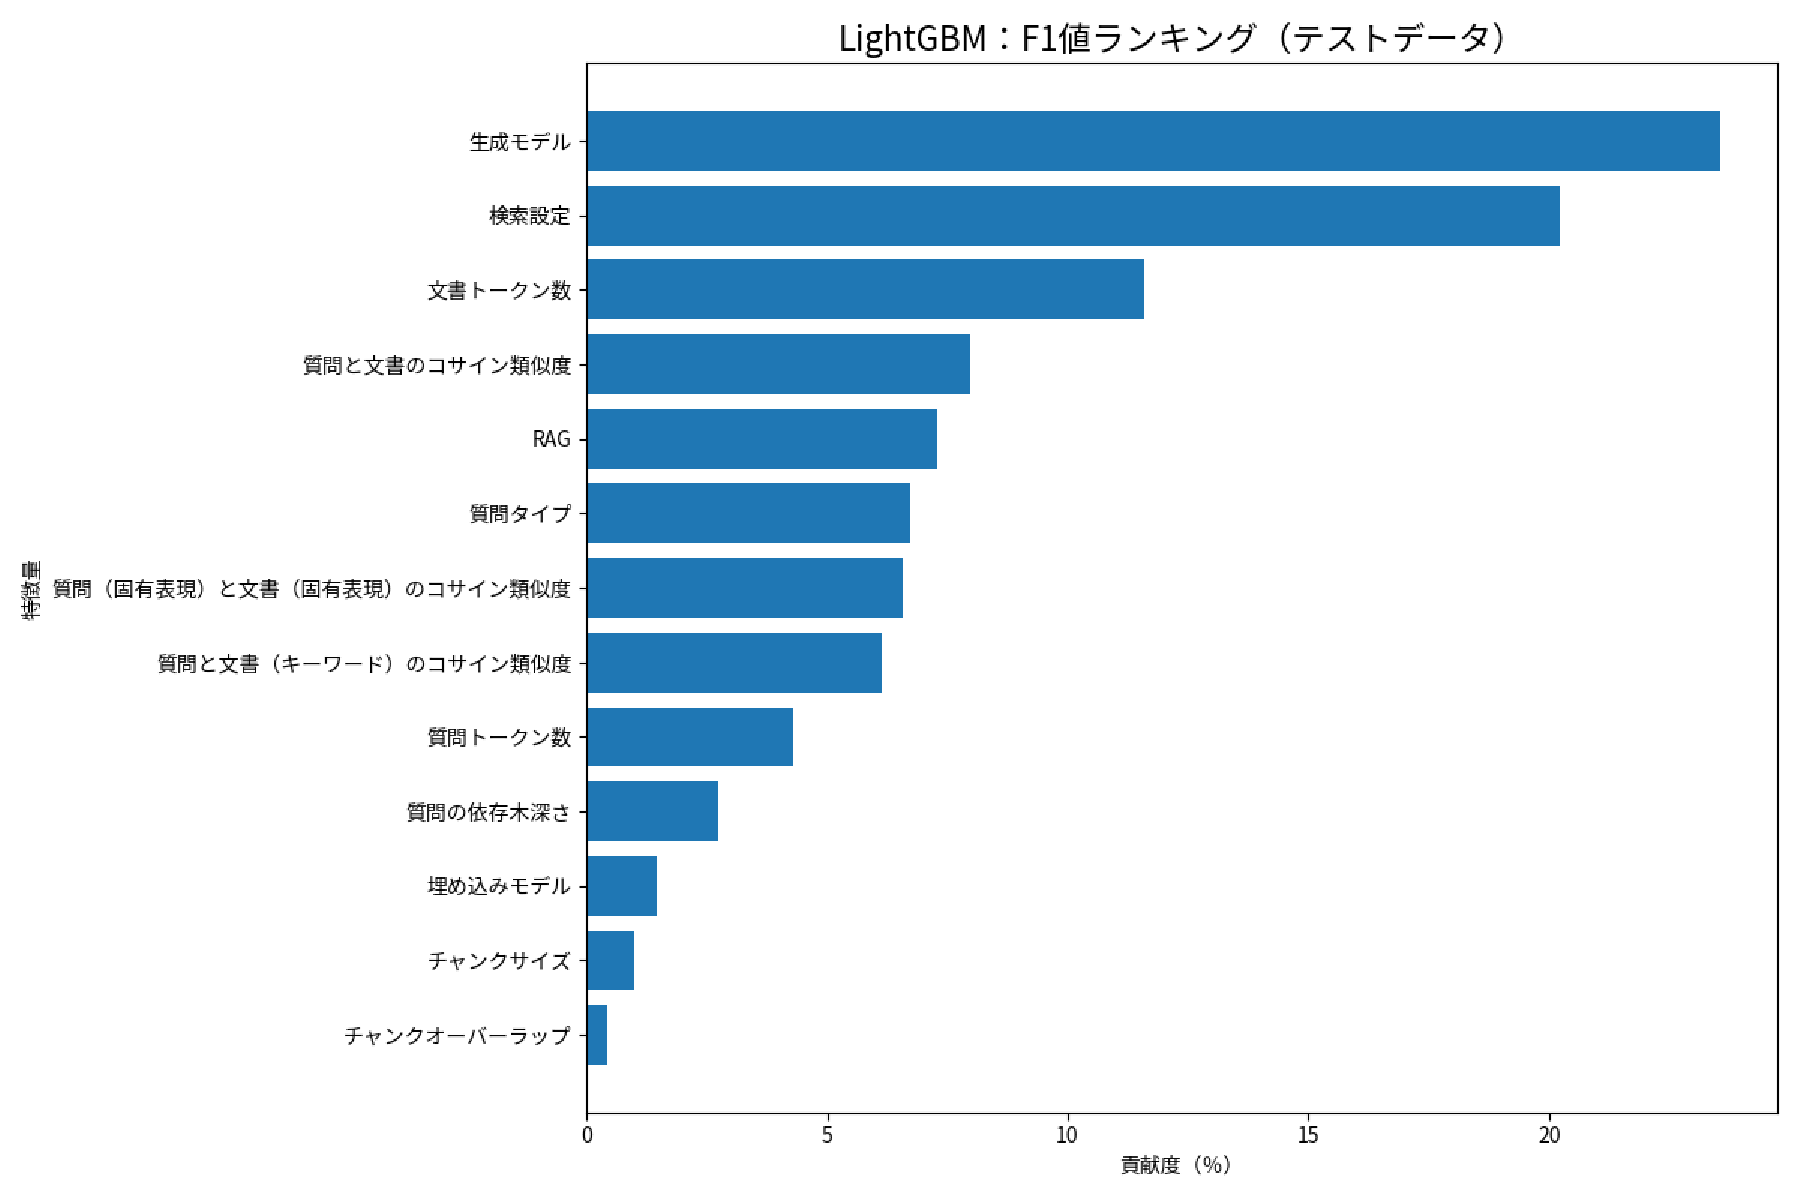
\includegraphics[width=\linewidth]{figures/feature_importance_f1_LightGBM_final.pdf}}
% \caption{$F_1$値ランキングにおける特徴量の貢献度}
% \label{feature_importance_f1_LightGBM_final}
% \end{figure*}

\subsection{定性分析} \label{sec5.7}
二つの質問応答例を用い，提案手法の挙動と失敗要因を定性的に分析する．
まず，映画監督の卒業大学を問う質問「Where did the director of film Nalini By Day, Nancy By Night graduate from?」を例に挙げる．
最頻出設定では「temple university」が得られ，提案@1でも同様に「temple university」を出力した．
続く提案@2から@4の設定も同様にNaiveRAGベースの構成であり，同様の誤答が出力された．
一方で，提案@5には異なる設定が含まれ，その実行結果として「mount holyoke college」のような正解となる回答が生成された．
これは，上位候補を広げるほど探索空間が拡大するためで，提案手法は固定のRAG構成では得ることのできない別回答を，候補集合として提示可能であることを示した．

次に，映画監督の死亡時期を比較する質問「Which film has the director died later, The Life And Loves Of Tschaikovsky or Dokuz Dağın Efesi?」を例に挙げる．
オラクルではGraphRAG構成で最大となる$F_1$値を示したが，$F_1$値RMはNaiveRAG構成を上位と予測した．
本質問は時系列的な事実照合を要し，複数文書間の関係をたどる必要がある．
GraphRAGは文書間関係を表現できるため，本来はこの種の質問に適する．
一方で，NaiveRAGは局所的な文脈一致に強く，質問と文中の単語レベルの類似度が高い場合に過大評価される傾向がある．
RMがコサイン類似度やトークン数といった特徴に影響され，GraphRAGよりもNaiveRAGを誤って選択したと推察される．

\subsection{本研究の限界} \label{sec5.8}
本研究では，RM学習により低コストかつ適応的なRAG構成選択を実現したが，以下の限界がある．

第一に，本手法は質問と文書の表層的および意味的特徴量である計7種を採用した．
定性分析の結果，高度な時系列推論や複数文書にまたがる複雑な論理構造を要する質問に対し，RMがNaiveRAGを誤選択する事例を確認した．
これは，現在の特徴量が語彙的類似性や文構造の深さに依存しており，知識グラフの構造的な適合性を評価できていないことに起因する．

第二に，本手法は実行時間の短縮において，オラクルに近い性能を達成した．
一方で，適合率や$F_1$値の最大化については，依然としてオラクル構成との間に有意な差がある．
96通りの構成空間において，精度を最大化する構成が局所的であり，現在のRM学習ではこれらを捉えきれていない可能性が高い．

第三に，大規模な実測データを効率的に収集するため，自動評価指標であるBERTScoreを用いた．
BERTScoreは意味的な類似性の評価に優れるが，コンテキストの忠実性やハルシネーションの有無を直接的には評価しない．
そのため，RMが事実とは異なる回答を生成する構成を高く評価するリスクを排除できていない．

第四に，本実験はSQuADおよびHotpotQAなどの一般的なドメインを用いて検証したが，医療，法務，社内文書といった専門性の高いドメインにおける有効性は未検証である．
文書の専門性や用語の特異性が高い場合，現在の埋め込みモデルに基づく意味的特徴量が機能しない可能性がある．
また，本手法はオフライン学習を対象としているため，未知のドメインデータを追加した際の有効性は保証されない．
% \section{本研究の限界} \label{sec6}
\section{おわりに} \label{sec6}
本研究では，質問に応じてRAGの構成を適応的に選択し，精度とコストのトレードオフを調整する手法を提案した．
具体的には，複数のRAG構成に対してRM学習を適用し，質問特徴，文書特徴，構成情報から有用なRAG構成を上位に提示するモデルを構築した．
その上で，適合率，再現率，$F_1$値，実行時間を重み付きで統合した評価指標に基づき，最終的な構成を選択する手法を設計した．
運用上の要求に応じて重みを変更することで，精度重視やコスト重視といった方針の切り替えが可能となった．
評価項目(ii)における性能評価では，全クエリに同一のRAG構成を適用する固定構成（標準設定・最頻出設定）や，既存の代表的な適応的RAG手法であるAdaptive-RAGと比較して，回答精度（BERTScore $F_1$値，EM，Token-level $F_1$値）の大幅な改善と実行時間の短縮（Pareto改善）を確認した．
さらに，Wilcoxon符号付き順位検定により，提案手法のベースラインに対する統計的有意な優位性を立証した．
次に，提示された上位候補からユーザが最終選択を行う評価項目(iii)では，すべての候補を試行する累積コストが発生するものの，精度がさらに向上し，時間重視方針においてはオラクルの時間最良設定と完全に一致するコスト最小化を達成した．
アブレーション分析により特徴量の重要度および提案手法全体の有効性を確認し，特徴量貢献度分析により生成・検索モデルなどのマクロ要素に加えてコサイン類似度やトークン数といったデータ依存の特徴量がランキング予測に強く寄与していることを明らかにした．

今後の課題は，RM（ランキングモデル）の予測精度のさらなる向上，および現在は手動で行っている優先度重みの自動推定メカニズムの構築である．具体的には，入力クエリの難易度やシステムの実行時制約から，重みベクトルを自動決定するゲートネットワークの設計などが挙げられる．

% 今後の課題は，RMの精度向上，ユーザ意図から重み設定の自動化，および評価指標の拡張である．

% \section{今後の課題} \label{sec6.2}
% 本研究の枠組みは有効性を示した一方で，オラクルの適合率最良構成，再現率最良構成，$F_1$値最良構成との差が残り，実用化に向けて複数の課題がある．

% 第一に，ランキングモデルの精度の向上が必要である．
% 精度指標を目的変数とした場合，生成の揺らぎや取得文書の質のばらつきにより順位が不安定になりやすい．
% そのため，学習データの拡充やモデル設計の改善に加え，複数回実行による期待値推定や不確実性を考慮した学習といった，評価のばらつきを前提とした頑健な順位学習が求められる．

% 第二に，候補設定集合の設計と探索範囲の最適化が課題である．
% 候補集合が有限である以上，理想設定が候補外に存在すれば上界に到達できない．
% その一方で，候補数が増加すると学習難度と運用負荷が増大する．
% したがって，多様性を確保しつつ冗長性を抑えた候補設計や，段階的に候補を広げる探索戦略を導入する必要がある．
% また，将来的には検索戦略，再ランキング，生成手順といった，より高次の設計要素を含めた適応化も検討課題となる．

% 第三に，重み設定の自動化とユーザ意図への適応が挙げられる．
% 本研究では重みを手動で設定した．
% しかし，実運用ではタスクや状況により要求が変化する．
% そのため，質問特性や環境制約から重みを推定する仕組み，あるいは少数のプリセットに整理したインタフェース設計が必要である．

% 第四に，上位$k$候補を用いる運用では，最終的に採用された設定の時間だけでなく，候補を複数回試行する総コストが重要となる．
% 今後は総コストを評価に含め，閾値に基づく早期終了といった段階的運用を含めた最適化が求められる．

% 第五に，評価指標の拡張が必要である．
% 本研究は適合率・再現率・$F_1$値と時間を中心に評価した．
% しかし，RAGの実運用では事実性や根拠の正確性といった，信頼性に直結する品質要因が重要である．
% 人手評価や根拠整合性評価を取り込み，目的変数として扱うことで，より実問題に即した適応的選択が可能になると考えられる．

% 以上の課題に取り組むことで，本研究の提案手法は，高精度側の上界に近づきつつ，総コスト制約下でも運用可能な適応的RAG選択手法として発展すると期待される．


% 謝辞
\begin{acknowledgment}
本研究成果の一部は，国立研究開発法人新エネルギー・産業技術 総合開発機構(NEDO)の委託業務(JPNP20006, JPNP25006)の結果得られたものです．
本研究はJSPS科研費 23K11221，25K03232 の助成を受けたものです．
\end{acknowledgment}

\bibliography{references}
\bibliographystyle{jsai}

\begin{biography}
\profile{n}{穴口 史将}{2024年青山学院大学理工学部情報テクノロジー学科卒業．同年6月から2026年3月まで，産業技術総合研究所リサーチアシスタント．同年同大学院理工学研究科前期博士課程修了．在学時に本研究に従事．現在に至る．言語処理学会の会員．}{photos/anaguchi}
% \newpage

\profile{n}{チャクラボルティ シュデシナ}{2023年カナダのウェスタンオンタリオ大学医学部神経科学プログラム大学院博士課程修了．同年，ウェスタンオンタリオ大学Robart Research Institute客員研究員．2024年より青山学院大学理工学部情報テクノロジー学科助教．現在に至る．博士（神経科学）．脳MRI画像を用いた認知神経科学研究に従事．Organization for Human Brain Mappingの会員．}{photos/SC}

\profile{m}{森田 武史}{2008年慶應義塾大学大学院理工学研究科後期博士課程修了．同年，日本学術振興会特別研究員(PD)．2009年慶應義塾大学大学院理工学研究科特別研究助教．2011年青山学院大学社会情報学部助手．2014年同助教．2015年慶應義塾大学理工学部管理工学科専任講師（有期）．2019年同准教授（有期）．2020年より青山学院大学理工学部情報テクノロジー学科准教授．2023年同教授．現在に至る．2022年より産業技術総合研究所人工知能研究センターの招聘研究員を兼任．博士（工学）．セマンティックWebとオントロジーに関する研究に従事．情報システム学会，ACM，日本データベース学会，電子情報通信学会，情報処理学会，言語処理学会の各会員．}{photos/morita}

\profile{m}{太田 葵}{2025年東京都立大学システムデザイン研究科情報科学域博士前期課程修了．同年より産業技術総合研究所人工知能研究センター研究員．現在に至る．修士（工学）．LLMエージェントやVQAに関する研究に従事．言語処理学会の会員．}{photos/ohta}

\profile{n}{浅田 真生}{2022年豊田工業大学大学院情報援用工学博士後期課程修了．2023年より産業技術総合研究所人工知能研究センター研究員．現在に至る．博士（工学）．専門は自然言語処理，情報抽出，拡散言語モデル．言語処理学会の会員．}{photos/asada}

\profile{m}{江上 周作}{2018年日本学術振興会特別研究員(DC2)．2019年電気通信大学大学院情報理工学研究科博士後期課程修了．同年海上・港湾・航空技術研究所研究員．2020年より産業技術総合研究所研究員．2023年より同研究所人工知能研究センター主任研究員．現在に至る．2019年より法政大学理工学部兼任講師，2023年より電気通信大学大学院情報理工学研究科連携准教授を兼任．博士（工学）．セマンティックWeb，オントロジー，知識グラフの構築と活用の研究に従事．2018年度，2022年度人工知能学会研究会優秀賞．2022年度同学会全国大会優秀賞．ISWC2021 Best Poster Award．言語処理学会，情報処理学会，IEEE，ACM，IAOAの各会員．}{photos/egami}

\profile{m}{鵜飼 孝典}{1992年3月東京工業大学大学院理工学研究科修士課程修了．2013年東京工業大学大学院情報理工学研究科博士課程修了.1992年より現在に至るまで富士通株式会社研究員. 博士(工学). 専門は知識グラフ，グラフ・ニューラル・ネットワーク，要求工学．ACM，情報処理学会の各会員．}{photos/ugai}

\profile{m}{濱崎 雅弘}{2005年総合研究大学院大学博士後期課程修了．博士（情報学）．同年より産業技術総合研究所特別研究員．現在，産業技術総合研究所人工知能研究センター副研究センター長．2017年より筑波大学連携大学院准教授を兼任．人工知能学会，情報処理学会，ACM各会員．ウェブ情報学，オンラインコミュニティの研究に従事．}{photos/hamasaki}
\end{biography}
\end{document}
